\documentclass{article}
\usepackage{lmodern}
\usepackage[T1]{fontenc}
\usepackage{shapepar}
\usepackage{microtype}
\usepackage{lipsum}
\usepackage{pgfplots}
\pgfplotsset{compat=1.9}
\usepackage{tikz}
\usetikzlibrary{calc,fit,intersections,folding}
\usepackage{pstricks-add}
\usetikzlibrary{arrows.meta,angles,arrows,quotes,backgrounds}
\usepackage[top = 5mm, bottom = 15mm]{geometry}

\newcommand{\clrone}{blue!90!black}
\newcommand{\clrtwo}{red!90!black}
\newcommand{\clrthree}{green!90!black}

\begin{document}\thispagestyle{empty}
    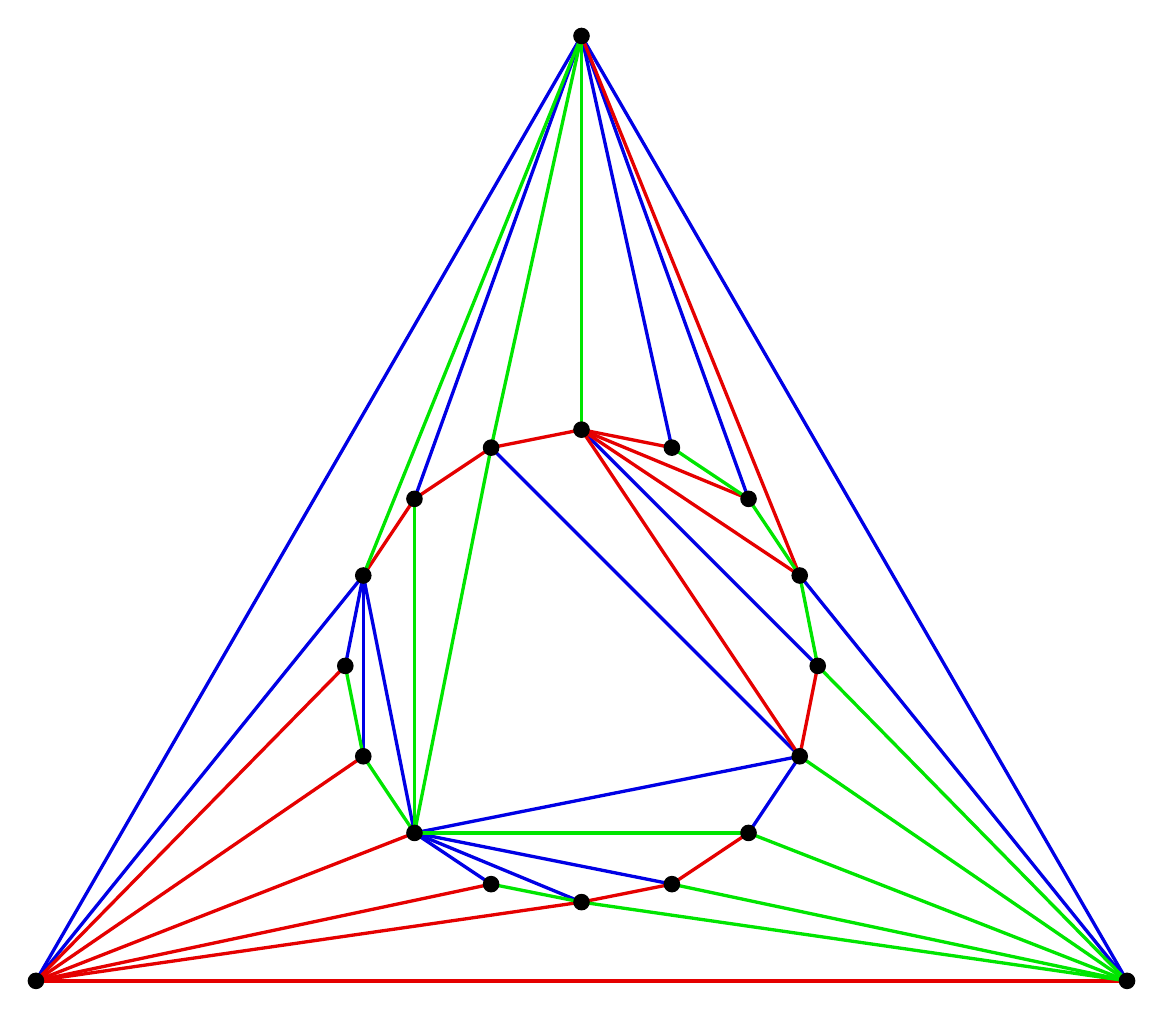
\begin{tikzpicture}

        \foreach\a in {0,1,2} {
            \coordinate (o\a) at (90+\a*120:8);
        }

        \foreach\a in {0, ..., 15} {
            \coordinate (i\a) at (90+\a*22.5:3);
        }

        \foreach \v/\w in {o0/o2, o0/o1, o0/i14, o0/i15, o0/i2, i3/i4, i3/i5, i3/i6, i6/i9, i6/i11, i10/i11, i1/i11, i6/i8, o2/i13, o1/i3, i6/i7, i12/i0} 
        {
            \draw[very thick, \clrone] (\v) -- (\w);
        }
        
        \foreach \v/\w in {o1/o2, o1/i5, o1/i7, o1/i8, i8/i9, i9/i10, i3/i2, i2/i1, i1/i0, i0/i15, i0/i14, i0/i13, i0/i11, i11/i12, o0/i13, o1/i4, o1/i6} 
        {
            \draw[very thick, \clrtwo] (\v) -- (\w);
        }
        
        \foreach \v/\w in {o2/i12, o2/i11, o2/i10, o2/i9, o2/i8, i10/i6, i8/i7, i6/i5, i5/i4, i6/i2, i6/i1, i15/i14, i14/i13, o0/i1, i12/i13, o0/i3, o0/i0} 
        {
            \draw[very thick, \clrthree] (\v) -- (\w);
        }

        \foreach\a in {0,1,2} {
            \fill (o\a) circle (3pt);
        }

        \foreach\a in {0, ..., 15} {
            \fill (i\a) circle (3pt);
        }

        
    \end{tikzpicture}

\end{document}
